%% Based on a TeXnicCenter-Template by Gyorgy SZEIDL.
%%%%%%%%%%%%%%%%%%%%%%%%%%%%%%%%%%%%%%%%%%%%%%%%%%%%%%%%%%%%%

%------------------------------------------------------------
%
\documentclass{article}%
%Options -- Point size:  10pt (default), 11pt, 12pt
%        -- Paper size:  letterpaper (default), a4paper, a5paper, b5paper
%                        legalpaper, executivepaper
%        -- Orientation  (portrait is the default)
%                        landscape
%        -- Print size:  oneside (default), twoside
%        -- Quality      final(default), draft
%        -- Title page   notitlepage, titlepage(default)
%        -- Columns      onecolumn(default), twocolumn
%        -- Equation numbering (equation numbers on the right is the default)
%                        leqno
%        -- Displayed equations (centered is the default)
%                        fleqn (equations start at the same distance from the right side)
%        -- Open bibliography style (closed is the default)
%                        openbib
% For instance the command
%           \documentclass[a4paper,12pt,leqno]{article}
% ensures that the paper size is a4, the fonts are typeset at the size 12p
% and the equation numbers are on the left side
%
\usepackage{amsmath}%
\usepackage{amsfonts}%
\usepackage{amssymb}%
\usepackage{graphicx}
\usepackage{float}
\usepackage{graphicx}
\usepackage{caption}
\usepackage{subcaption}
\usepackage{float}
\usepackage{authblk}
\usepackage{booktabs}
%-------------------------------------------
\newtheorem{theorem}{Theorem}
\newtheorem{acknowledgement}[theorem]{Acknowledgement}
\newtheorem{algorithm}[theorem]{Algorithm}
\newtheorem{axiom}[theorem]{Axiom}
\newtheorem{case}[theorem]{Case}
\newtheorem{claim}[theorem]{Claim}
\newtheorem{conclusion}[theorem]{Conclusion}
\newtheorem{condition}[theorem]{Condition}
\newtheorem{conjecture}[theorem]{Conjecture}
\newtheorem{corollary}[theorem]{Corollary}
\newtheorem{criterion}[theorem]{Criterion}
\newtheorem{definition}[theorem]{Definition}
\newtheorem{example}[theorem]{Example}
\newtheorem{exercise}[theorem]{Exercise}
\newtheorem{lemma}[theorem]{Lemma}
\newtheorem{notation}[theorem]{Notation}
\newtheorem{problem}[theorem]{Problem}
\newtheorem{proposition}[theorem]{Proposition}
\newtheorem{remark}[theorem]{Remark}
\newtheorem{solution}[theorem]{Solution}
\newtheorem{summary}[theorem]{Summary}
\newenvironment{proof}[1][Proof]{\textbf{#1.} }{\ \rule{0.5em}{0.5em}}

\begin{document}
\title{ Title }
\author[]{ Author}
\affil{ Affiliation }
\affil{\textit {email}}
\maketitle

\newpage

\begin{abstract}

NEREID is a bundle of projects shared between TUM and INSA Lyon. \\

Our project is a bit peculiar. We are meant to improve Evince, the default PDF
reader on Linux (that also works on Windows).\\

With the initial project, we intended to improve annotations, mainly addind
embedded highlighting. This was already done by someone at \emph{Google Summer
of code}, therefore we decided to work on hypertext link navigation. We are
strongly commited to having the features be accepted by the community. \\

Being an open-source project, it will be a great experience, which will get a
better understanding of the open-source ecosystem. The project also follows up
our engineering courses, at TUM as well as at INSA Lyon. Moreover, the code
itself is very advanced and will enhance our programming skills.

\end{abstract}

\section{Story Line}
Every week we hold a meeting on "Skype"; in this meeting we distribute new tasks, we process the quality of what we've done during the prevoius week and share our new findings about each part of the project with other members.

We use "Trello" as a collaboration tool and task distributer that organizes our project into cards. It provides us an overview on what's being worked on, who's working on what, and where something is in a process.

The first step for all of us was compiling the project on our systems. This part was a bit challenging as it requires many libraries and dependencies. Then we tried to get familiar with the code. The next step was one of the most important parts, to choose useful and inovative features in order to implement. All team members searched and studied about it and finally we asked the community to confirm the most relevant and we started to distrubte the tasks for that specific feature.

\section{Project Planning and Management}
Complex projects usually involve highly qualified specialist project managers. We are trying following tools for our project management.
\begin{enumerate}
\item Work Breakdown Structure: 
We planned start by breaking down the overall objective into smaller packages, until each parcel 
of work is self-contained and can be attributed to one or more than one team members.
\item Dependencies: 
We list the tasks and which depend on the completion of which before they can begin. At this 
point we can also estimate how long each will take. 
This kind of analysis allows projects to be planned to make the most effective use of time and 
resources, and to deliver key outcomes and milestones to a specific timetable. 
\end{enumerate}

\section{Quality Process}
Every software development needs to be focused on the delivery of quality. One of the most important customer service skills is the ability to understand and effectively respond to the customer’s needs and concerns. Quality process must be a part of the entire software development life cycle (SDLC) from inception through implementation.

We see quality process fundamentally as a way of solving problems. Once we sense a problem, good problem solving technique involves alternating between the levels of thought and experience. For instance, after we sense a problem, we should collect some data to get insight regarding the area of the problem,
choose the specific relevant improvement activity we will undertake, collect some more
data, analyze the data to find the causes of the problem, plan a solution and try it, collect
some more data to evaluate the effects of the new solution, standardize on the solution if
it works, and conclude by reflecting on what we did.

We use the following steps to ensure that we measure the right quality-control factors in the right way.
\begin{itemize}
\item Determine what to measure.
\item Determine our measurement process by selecting the best process for our needs.
\item Define exactly how we'll use the selected measurement process.
\item Perform the measurements and compare to customer specifications.
\item Confirm the quality of our data with compare-and-review checks and the help of a computer.
\item Make sense of our data with coding and different data charts.
\end{itemize}

\section{Risk Management}
\subsection{Risk Factors}

\begin{description}
\item[Technical issues] The specificity of the field of study requires
strong specialization of the team members.
\item [Degree of integration and project size] The project is ambitious.
Its scale suggests a modular architecture
resulting in strong dependencies and interactions. \\
It will be necessary to be rigorous and consistent to face them, 
so we decided to use Agile development methods (such as Scrum).
\item [Team Instability] Mutual emulation is necessary to
prevent any down-spirit in the team.
\end {description}

\subsubsection {Organizational Configuration}

\begin {description}
\item [Groupwares] Establishment of standards, styleguide,
graphic charter and collaborative tools. We define classic
workflow of the production cycle and the validation of a deliverable.
\item [Maturity] It is necessary to set up a regular monitoring
planning and a wide frame. The project managers and
quality assessers should regularly monitor compliance with
deadlines and anticipate the next ones.
\end {description}

\subsection {Project Risks}

\begin {description}
\item [Financial risks] In this case, this is an analogy for
the amount of work. It is the responsibility of the
project leaders to carry out a strict planning structured by a
regular monitoring of the work on each task. It will be necessary
to provide meaningful indicators of these aspects on
project monitoring dashboards.
\item [Human risks] Possible cases of incompetence will be notified by
the allocation of technology watch slots, and the use of
systematic mutual assistance.
\item [Technological risks] To prevent the loss of documents, a
Version Manager will be used consistently (Google Drive and Git).
\end {description}

\section{Task weight}

\begin{tabular}{|l|c|}
\hline
Technical specification & 12h \\ \hline
Implement software tests & 8h \\ \hline
Compile up-to-date Evince code & 6h \\ \hline
Call another app from the code (Linux) & 4h \\ \hline
Find out a link is a link & 4h \\ \hline
Integrate the POCs into Evince last up-to-date code & 4h \\ \hline
Make a link clickable & 4h \\ \hline
Cross-platform investigation & 4h \\ \hline
Clear Git & 3h \\ \hline
Description of every task & 2h \\ \hline
Project management documentation & 2h \\ \hline
Stakes of international work & 2h \\ \hline
Check out the validation process & 2h \\ \hline
Preparing Slides & 2h \\ \hline
Check out the test process & 2h \\ \hline
Introduction and Storyline & 1h \\ \hline
Check dependencies between tasks & 1h \\ \hline
\end{tabular}

\begin{figure}[ht]
    \centering
    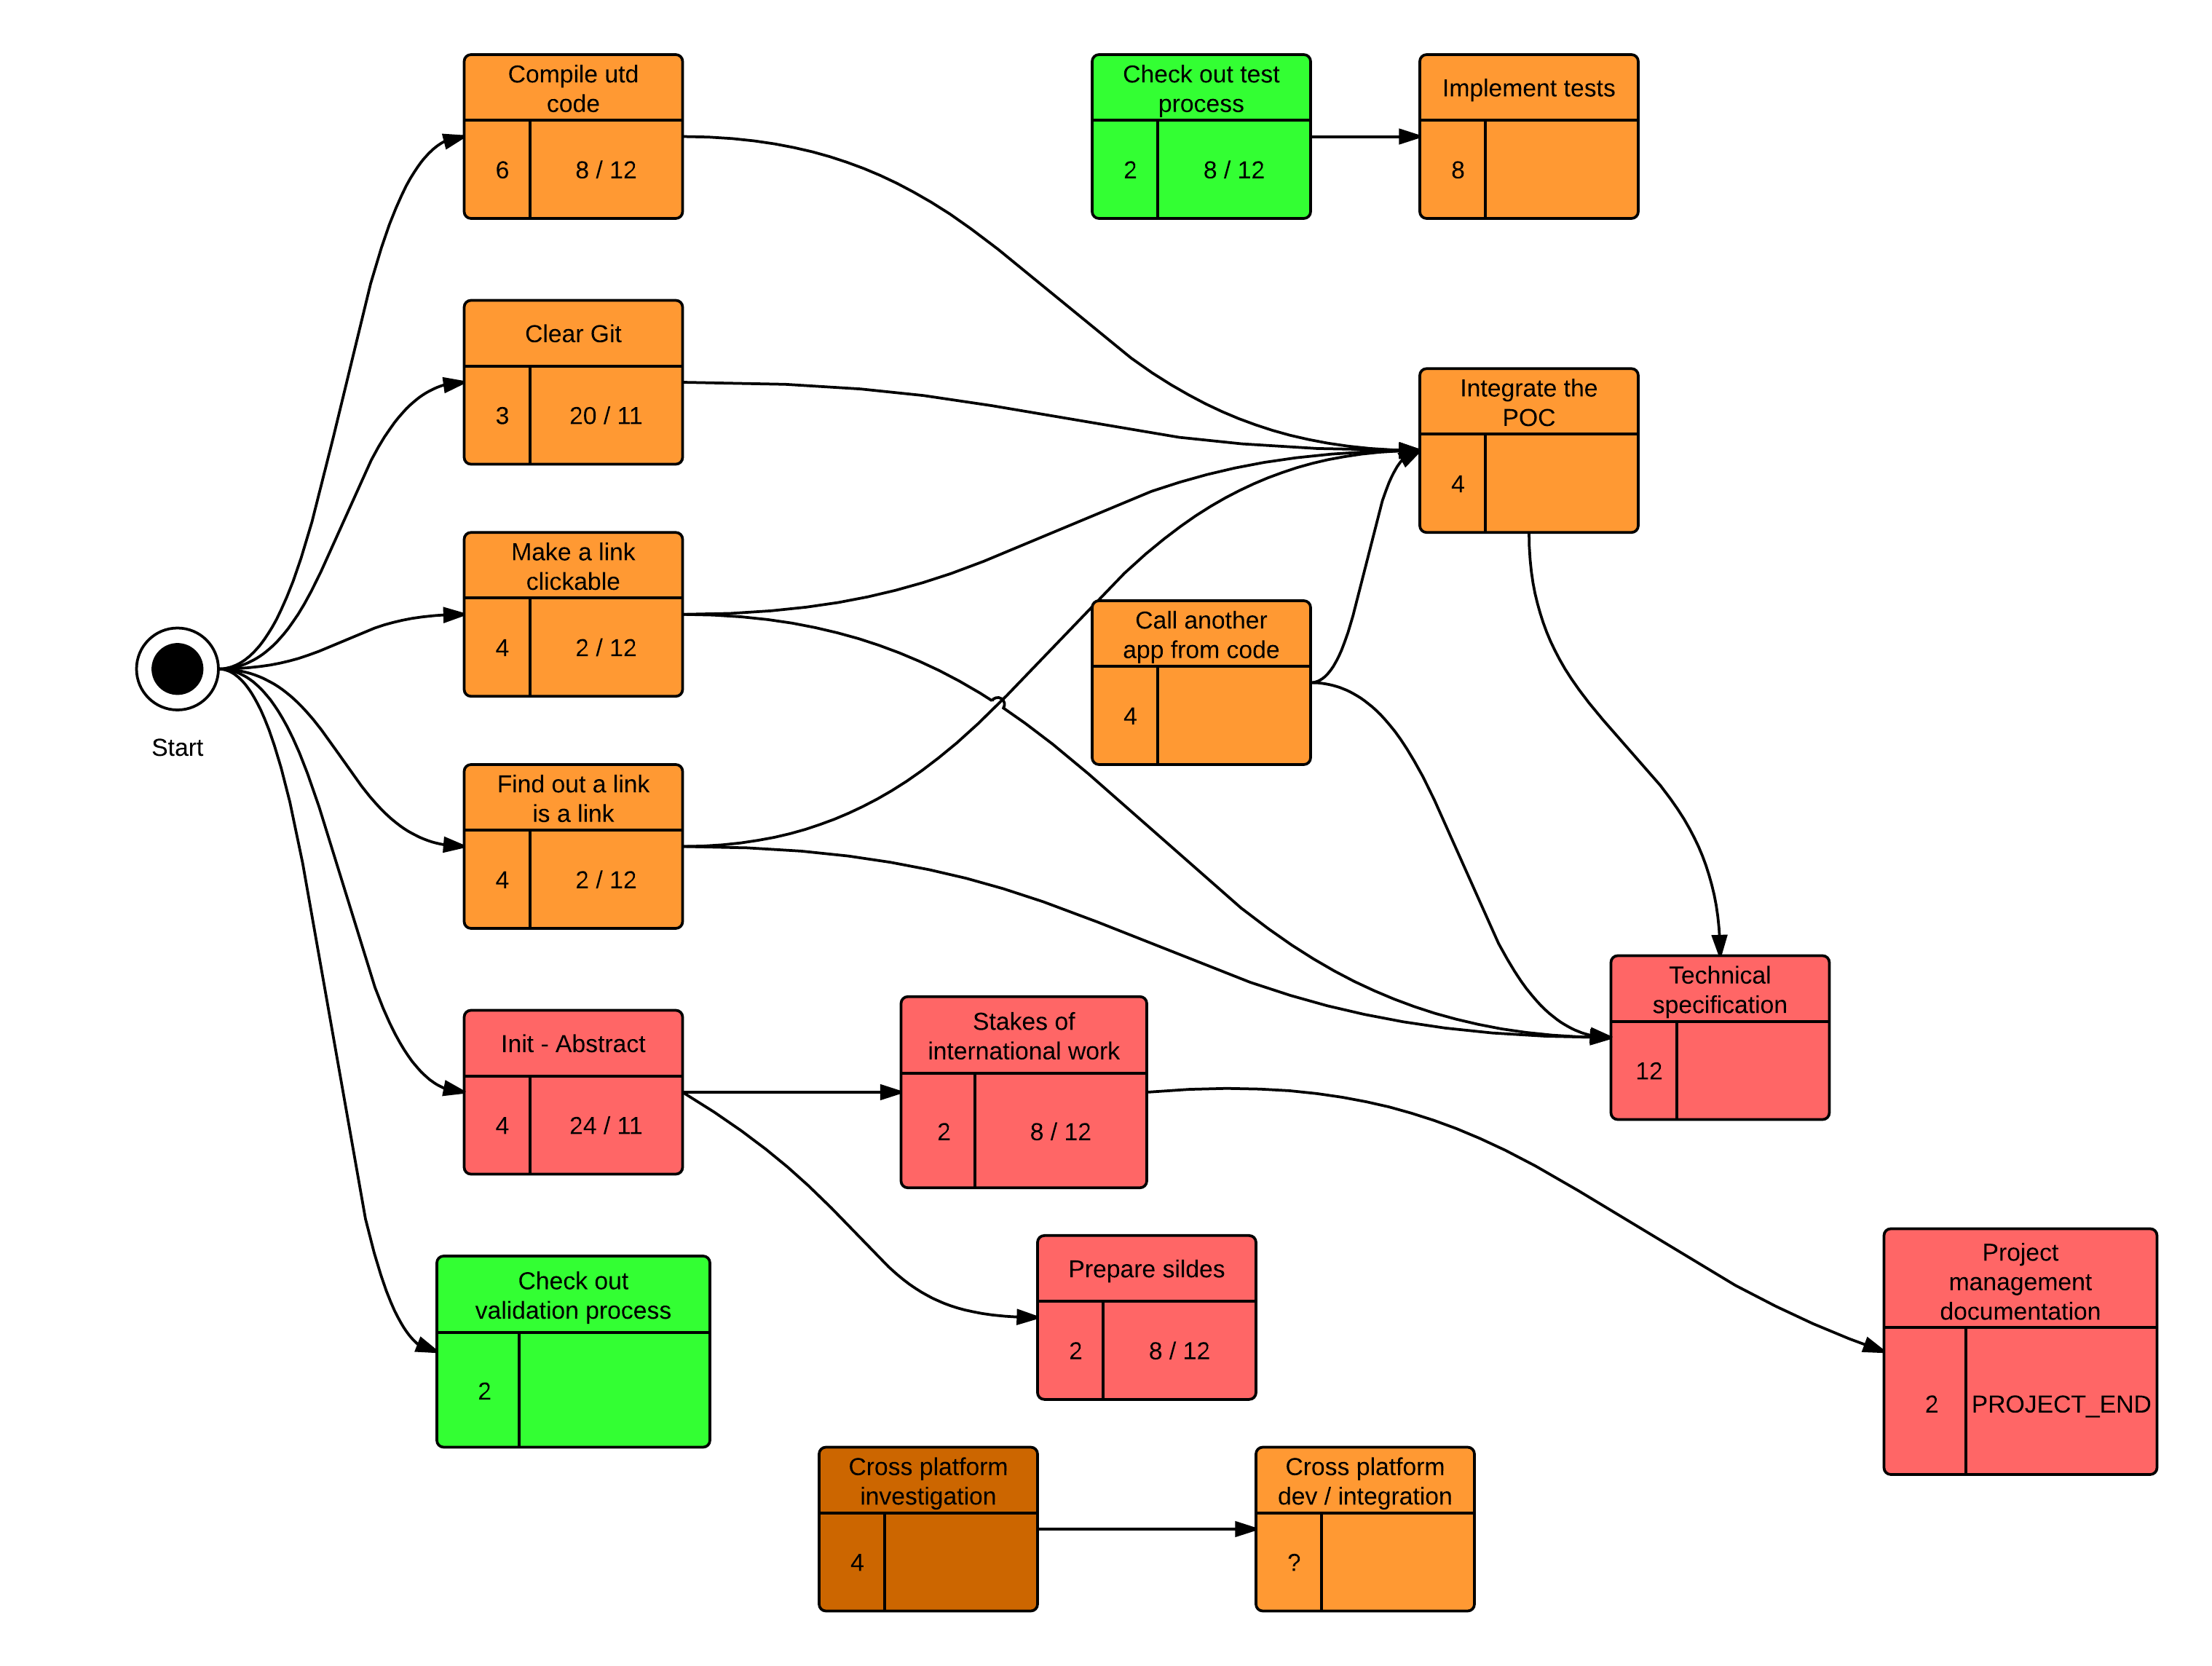
\includegraphics[width=0.5\paperheight]{gantt}
    \caption{Previsional organization}
    \label{fig:gantt}
\end{figure}

\section{Task Distribution}
% Please add the following required packages to your document preamble:
% \usepackage{graphicx}
\begin{table}[h]
\centering
\caption{Implementation tasks}
\label{my-label}
\resizebox{\textwidth}{!}{%
	\begin{tabular}{|l|l|l|l|l|}
	\hline
	\textbf{Tasks} & \textbf{Adrian Delmarre} & \textbf{Shabnam Najafian} & \textbf{Quentin Coursodon} & \textbf{Mohammad Mahadi Hasan} \\ \hline
	\textbf{Call another app from the code (Linux)} &  & $\surd$ & $\surd$ &  \\ \hline
	\textbf{Integrate the POCs into Evince last up-to-date code} & $\surd$  &  & $\surd$ &  \\ \hline
	\textbf{Implement software tests} & $\surd$  &  &  & $\surd$ \\ \hline
	\textbf{Find out a link is a link} &  &  & $\surd$  & $\surd$ \\ \hline
	\textbf{Make a link clickable} & $\surd$ & $\surd$ &  &  \\ \hline
	\textbf{Compile up-to-date Evince code} & $\surd$ & $\surd$ &  &  \\ \hline
	\end{tabular}
}
\end{table}

% Please add the following required packages to your document preamble:
% \usepackage{graphicx}
\begin{table}[h]
\centering
\caption{Documentation tasks}
\label{my-label}
\resizebox{\textwidth}{!}{% Ÿøłø
	\begin{tabular}{|l|l|l|l|l|}
	\hline
	\textbf{Tasks} & \textbf{Adrian Delmarre} & \textbf{Shabnam Najafian} & \textbf{Quentin Coursodon} & \textbf{Mohammad Mahadi Hasan} \\ \hline
	\textbf{Discribtion of every task} & $\surd$ & $\surd$ & $\surd$ & $\surd$ \\ \hline
	\textbf{Introduction and Story line} & $\surd$ & $\surd$ &  &  \\ \hline
	\textbf{Check dependencies between tasks} &  &  &  &  $\surd$\\ \hline
	\textbf{Technical specification} & $\surd$ & $\surd$ & $\surd$ & $\surd$ \\ \hline
	\textbf{Project management documentation} & $\surd$ & $\surd$ &  &  \\ \hline
	\textbf{Stakes of international work} & $\surd$ & $\surd$ & $\surd$ & $\surd$ \\ \hline
	\textbf{Preparing Slides} & $\surd$ & $\surd$ & $\surd$ & $\surd$ \\ \hline
	\end{tabular}
}
\end{table}

% Please add the following required packages to your document preamble:
% \usepackage{graphicx}
\begin{table}[h]
\centering
\caption{Architecture tasks}
\label{my-label}
\resizebox{\textwidth}{!}{%	
	\begin{tabular}{|l|l|l|l|l|}
	\hline
	\textbf{Tasks} & \textbf{Adrian Delmarre} & \textbf{Shabnam Najafian} & \textbf{Quentin Coursodon} & \textbf{Mohammad Mahadi Hasan} \\ \hline
	\textbf{Technical specification} & d & d & d & d \\ \hline
	\textbf{Cross-platform investigation} & d &  &  &  \\ \hline
	\textbf{Clear Git} &  &  & d &  \\ \hline
	\end{tabular}
}
\end{table}

% Please add the following required packages to your document preamble:
% \usepackage{graphicx}
\begin{table}[h]
\centering
\caption{Validation and Community tasks}
\label{my-label}
\resizebox{\textwidth}{!}{%
	\begin{tabular}{|l|l|l|l|l|}
	\hline
	\textbf{Tasks} & \textbf{Adrian Delmarre} & \textbf{Shabnam Najafian} & \textbf{Quentin Coursodon} & \textbf{Mohammad Mahadi Hasan} \\ \hline
	\textbf{Check out the validation process} & d & d &  & d \\ \hline
	\textbf{Check out the test process} &  & d &  & d \\ \hline
	\end{tabular}
}
\end{table}



\end{document}
